% RiskPredictor research report. Compile: pdflatex report; bibtex report; pdflatex report; pdflatex report
\documentclass[11pt]{article}
\usepackage[margin=1in]{geometry}
\usepackage[T1]{fontenc}
\usepackage{lmodern}
\usepackage{microtype}
\usepackage{amsmath,amssymb}
\usepackage{booktabs,array}
\usepackage{graphicx}
\usepackage{float}
\usepackage{caption}
\usepackage{enumitem}
\usepackage{xcolor}
\usepackage[numbers,sort&compress]{natbib}
\usepackage[hidelinks]{hyperref}
\graphicspath{{figures/}}
\captionsetup{font=small,labelfont=bf}
\setlength{\parskip}{4pt}
\renewcommand{\arraystretch}{1.08}
\setcounter{secnumdepth}{3}
\setcounter{tocdepth}{2}
\newcommand{\aname}{\textit{RiskPredictor}}

\title{\aname: Pricing and Risk for Sports Prediction Markets\\[4pt]\large Research report}
\author{Sai Kishore Pachigolla\\ \small NYU Tandon, Finance and Risk Engineering \\ \small Advisor: Prof.\ Dennis Shasha, Courant Institute}
\date{Last updated: 21 October 2026}

\begin{document}
\maketitle

\begin{abstract}
\noindent Prediction markets on sporting events now trade billions of contracts a season, yet the risk tools of traditional finance assume continuous prices and long histories that binary, short-lived contracts do not have. This report records a project to build a risk engine for such markets. Its central idea is that a contract's price is a probability, so pricing and settlement risk are the same calculation, and a joint model over a game's final score prices every contract on the game consistently and lets risk net across them. So far we have classified which traditional risk tools carry over; surveyed the literature on predicting NFL games; built a leak-free table of 759 pre-game features for 7,548 games (1999--2026); and fitted a two-output random forest that predicts both teams' scores. Evaluated walk-forward over sixteen seasons it predicts the margin with a mean absolute error of 10.35 points, against 10.38 for Elo and 10.05 for the Vegas closing line, matching the published literature. Its score predictions are calibrated, its residuals are uncorrelated with standard deviations of 9.6 and 9.4 points, and, placed on an empirical score grid that preserves the NFL's key-number spikes, they price a game's full ladder of contracts to within a cent of the Kalshi order book. Ensembles with public forecasts do not beat the closing line. The engine's value therefore lies in a calibrated joint distribution rather than a better point forecast. The report is updated weekly; Section~\ref{sec:weekly} holds the dated progress reports.
\end{abstract}

\tableofcontents

% ===== sections/idea.tex =====
\section{The idea}\label{sec:idea}


Prediction markets have moved from a niche into the mainstream. On Kalshi alone the three main contract types on a single NFL week (game winner, point spread, game total) traded close to two billion contracts over the first three weeks of the 2026 season, and the Super Bowl winner market carries over a hundred million contracts of open interest. In this document we explore how the methods of traditional financial risk management apply to such markets and build a risk engine for them, \aname.

The goals of the engine are:
\begin{enumerate}[nosep]
\item compute security-level and portfolio-level risk;
\item in computing portfolio risk, add or net exposures according to the defined behaviour of the assets (netting through correlation, or, as we argue below, through a joint outcome model);
\item produce metrics that show what a book would actually do when the market moves;
\item at a later stage, support margin, collateral and leverage calculations;
\item identify cross-market hedging opportunities that allow more balanced products and portfolios.
\end{enumerate}

\subsection{A contract's price is a probability, so pricing and risk are one model}\label{sec:pricing}


A binary contract pays \$1 or nothing, so its fair value under any probability assessment $\pi$ of the outcome is $\pi$ dollars, and with only two outcomes that probability \emph{is} the full profit-and-loss distribution (Section~\ref{sec:binaryvar}). Pricing and settlement risk are therefore the same calculation. For a portfolio, the pricing model must be a joint one, because the joint probabilities are what allow risk to net across positions.

{\color{red}\textbf{Amine comment:} Please distinguish the model's outcome probabilities from market prices. Treating them as equal requires assumptions beyond accounting for fees and spreads. I believe matching prices alone does not show that the probabilities accurately describe future outcomes.}

{\color{blue}\textbf{Sai comment:} Fixed. The paragraph below now separates the market price $p$ from the model probability $\pi$, lists the assumptions under which they coincide, and states that outcome accuracy is judged only against results (Sections~\ref{sec:scoremodel} and~\ref{sec:w1021}), with price matching read as consistency with the market, not correctness.}

Two probabilities appear in this document and we keep them apart. The \emph{market price} $p$ of a contract is what the exchange's order book shows, net of fee and spread. The \emph{model probability} $\pi$ is our estimate of the chance the outcome occurs. The two coincide only under assumptions that go beyond fees: that the marginal trader is risk-neutral and uninformed traders' flow is absorbed without moving the price, and that the market is efficient in the sense that its price already uses all public information. Levitt~\cite{levitt2004} shows that sportsbooks deliberately set prices away from their own probabilities to exploit bettor biases, so even an informed price need not equal its setter's probability. We therefore use market prices for two purposes only: as a benchmark that any model must be compared with, and as the mark at which a position is valued before settlement. Whether model probabilities describe future outcomes is a separate question, answered only by comparing them with what happened: the calibration plots and Brier scores of Sections~\ref{sec:scoremodel} and~\ref{sec:w1021} do that, and the market's own prices are held to the same test in Figure~\ref{fig:kalshi_cal}. Matching Kalshi's prices, as in the worked example of Section~\ref{sec:w0930}, shows that a model is consistent with the market, not that either is right.

A proper joint outcome model, such as a distribution over the final score of a game, gives everything in Table~\ref{tab:joint_uses} at once.

\begin{table}[H]
\centering
\small
\begin{tabular}{p{6.5cm}p{6.5cm}}
\toprule
\textbf{Output} & \textbf{Used for} \\
\midrule
Fair price of every contract on the game & Pricing \\
Probability of each outcome state & ES, probability of loss, expected loss \\
Joint behaviour of contracts on the same game & Netting (goal 2 of the engine) \\
Consistent prices across winner, spread, total and props & Detecting mispricing between related contracts \\
\bottomrule
\end{tabular}
\caption{What a joint outcome model provides.}
\label{tab:joint_uses}
\end{table}

Every Kalshi contract on a game is a region of the final-score grid. With $h$ and $a$ the home and away scores, the winner contract pays when $h-a>0$ (ties settle at \$0.50), a spread contract at strike $k$ pays when $h-a>k$, and a total contract pays when $h+a>k$. One probability table $p(h,a)$ prices all of them by summing cells, and a book of positions is a payoff vector over the same grid.

{\color{red}\textbf{Amine comment:} Fitting spread and total prices does not establish how margin and total behave together.}

{\color{blue}\textbf{Sai comment:} Fixed. The paragraph below states that the ladders identify only the two marginals and that the dependence between margin and total is an assumption carried by the historical prior (parity, correlation 0.03, conditional widening), untestable against listed contracts.}

The listed contracts do not, however, identify the whole table. Every winner and spread contract is a function of the margin $h-a$ alone and every total contract of $h+a$ alone, so a game's full ladder of prices pins down the two marginal distributions and says nothing about how margin and total move together. The dependence between them has to come from somewhere else. In our construction it comes from the historical prior: the empirical score table carries the parity constraint (margin and total are always both odd or both even), the near-zero linear correlation between them (0.03 over 2015--2026) and the modest widening of the margin in high-scoring games, and the tilt of Section~\ref{sec:w0930} preserves all three because it only reweights cells. This is an assumption, stable across seasons in the data we have, not something the market confirms. It matters for any position whose payoff depends on both numbers at once, such as a spread and a total on the same game held together, and it could only be tested against contracts that pay on joint events (team totals, same-game parlays), which Kalshi does not list.

\subsection{VaR and expected shortfall for binary contracts}\label{sec:binaryvar}


For a binary contract none of the three traditional computations is needed, because the loss distribution can be written down. A position of $q$ contracts bought at price $p$ pays $q(1-p)$ if the event occurs and loses $qp$ otherwise. We define the loss as minus the profit, $L = -\text{P\&L}$, so a gain is a negative loss; if the probability of the event is $\pi$, $L$ takes the value $qp$ with probability $1-\pi$ and $-q(1-p)$ with probability $\pi$. With $\mathrm{VaR}_\alpha = \inf\{\ell : P(L\le \ell)\ge\alpha\}$ and $\mathrm{ES}_\alpha = \frac{1}{1-\alpha}\int_\alpha^1 \mathrm{VaR}_u\,du$,
\[
\mathrm{VaR}_\alpha = \begin{cases} qp & \text{if } \alpha > \pi,\\ -q(1-p) & \text{if } \alpha \le \pi,\end{cases}
\qquad
\mathrm{ES}_\alpha = \begin{cases} qp & \text{if } \alpha \ge \pi,\\[2pt] \dfrac{(1-\pi)\,qp - (\pi-\alpha)\,q(1-p)}{1-\alpha} & \text{if } \alpha < \pi.\end{cases}
\]
When the loss state is rarer than $1-\alpha$ (a likely event, $\pi>\alpha$), the $\alpha$-quantile of the loss is the gain state and VaR is negative; the tail average then mixes the loss state with part of the gain state. An earlier draft truncated gains at zero, $L^+=\max(L,0)$, which leaves VaR at $0$ rather than $-q(1-p)$ in that case and overstates ES by $(\pi-\alpha)\,q(1-p)/(1-\alpha)$; for the common case $\alpha\ge\pi$ the two conventions agree. So for a single contract the whole of risk measurement reduces to one number, $\pi$, which is also the fair price. For a portfolio of contracts on the same game the loss distribution is a sum over the joint outcomes of the game: with a probability table $p(h,a)$ over the final score, each position's payoff is a function of $(h,a)$, the portfolio profit and loss is their sum cell by cell, and VaR, ES, the worst case and the probability of loss are read directly from the resulting distribution with no simulation and no covariance matrix. This is the sense in which the pricing model and the risk model are the same object, and it is why the rest of this document is about building $p(h,a)$.
{\color{red}\textbf{Amine comment:} Please define loss explicitly. The formulas treat gains as zero; I believe defining loss as minus profit can give different VaR and expected shortfall values?}

{\color{blue}\textbf{Sai comment:} Fixed. Loss is now defined as $L=-\text{P\&L}$ and the VaR and ES formulas above are the signed-loss versions; the text notes where the earlier truncated-at-zero formulas differed (VaR of $0$ instead of $-q(1-p)$, and ES overstated by $(\pi-\alpha)\,q(1-p)/(1-\alpha)$, when $\pi>\alpha$).}

\subsection{Which traditional risk tools carry over}\label{sec:tools}


Traditional risk tools were built for instruments whose prices move continuously and have long histories. Sports prediction contracts pay exactly \$1 or \$0, last hours or days, and move in jumps. As a result the \emph{processes} of traditional risk management carry over, the \emph{measures} need adapting, and the \emph{statistical assumptions} no longer hold. Table~\ref{tab:tools} summarises our classification.

\begin{table}[H]
\centering
\small
\begin{tabular}{p{2.5cm}p{5.0cm}p{7.6cm}}
\toprule
\textbf{Category} & \textbf{Tools} & \textbf{Why} \\
\midrule
Works as-is & Expected shortfall, scenario revaluation, SPAN margining, stress testing, limit frameworks, counterparty exposure & They work for any payoff shape. Because every possible outcome can be listed, they can be computed exactly. \\
Needs adapting & Greeks, jump-to-default, basket correlation, netting, liquidity-adjusted risk, backtesting & The concepts are valid but must be reworked for binary, jump-driven payoffs, where dependence between contracts comes mostly from their structure rather than from statistics. \\
Does not work & VaR as usually computed, covariance matrices, factor models, historical price simulation, continuous hedging & They assume smooth, normally distributed returns with long price histories, none of which exist here. \\
New to prediction markets & Resolution-rule risk, cross-venue basis risk, integrity risk & These have no direct equivalent in traditional finance. \\
\bottomrule
\end{tabular}
\caption{Traditional risk tools and how they transfer to binary sports contracts.}
\label{tab:tools}
\end{table}

\subsubsection{Terms}

\begin{description}[nosep,leftmargin=0pt,labelindent=0pt]
\item[Value at Risk (VaR)] the loss that will not be exceeded at a given confidence level (e.g.\ 95\%). It ignores how large losses can be beyond that point.
\item[Expected shortfall (ES)] the average loss in the worst outcomes beyond the VaR threshold, which captures the size of the tail.
\item[Scenario revaluation] repricing every position under each possible scenario and adding up the profit and loss.
\item[SPAN margining] setting collateral equal to the worst portfolio loss across a defined set of scenarios.
\item[Stress testing] measuring losses under extreme but plausible events. \emph{Reverse} stress testing finds the events that would cause a given loss.
\item[Greeks] sensitivities of a position's value. \emph{Delta} measures the response to price, \emph{gamma} how delta itself changes, and \emph{theta} the effect of time passing.
\item[Basket correlation] risk in a product that depends on several events together (e.g.\ a parlay), driven by how those events are related.
\item[Netting] offsetting gains and losses across related positions to find the true combined exposure.
\item[Liquidity-adjusted risk] risk measured at the price one could actually exit at, rather than the mid-price.
\item[Covariance matrix, factor model] statistical tools that estimate how assets move together from historical returns.
\item[Counterparty exposure] potential loss if a counterparty or venue fails to pay.
\item[Resolution-rule risk] loss from how a contract settles, e.g.\ voids, pushes, overtime or stat corrections.
\item[Cross-venue basis risk] the ``same'' contract settling differently on two platforms.
\item[Integrity risk] loss from insider information or match-fixing.
\end{description}

\subsubsection{Value at Risk}

VaR answers one question: how much could I lose over a given period, at a given confidence level, under normal market conditions? Every VaR number has three parts: a loss amount, a time horizon and a confidence level. It is traditionally computed in one of three ways: parametrically, assuming a normal distribution of the underlying; by historical simulation; or by Monte Carlo. Its limitations are well known. It says nothing about the size of losses beyond the threshold, so two portfolios can have the same VaR while one loses ten times more in the worst 1\% of cases. It is not subadditive, so VaR$(A+B)$ can exceed VaR$(A)$ + VaR$(B)$, which makes diversification appear to increase risk; for this reason it is not a coherent risk measure in the sense of Artzner et al.~\cite{artzner1999}. And it relies on normal conditions, while correlations and volatilities shift sharply in a crisis.


% ===== sections/data.tex =====
\section{Data}\label{sec:data}

\subsection{Kalshi}

Kalshi is a regulated US exchange on which event contracts trade in a central limit order book, each contract paying \$1 if the event occurs. Table~\ref{tab:kalshi_series} lists the NFL contract series with their volume at the time of our first survey. Game-level contracts (winner, spread, total) are the focus of this project because they are the ones a joint score model prices directly.

\begin{table}[H]
\centering
\footnotesize
\begin{tabular}{llrrr}
\toprule
\textbf{Series} & \textbf{Type} & \textbf{Markets} & \textbf{Volume} & \textbf{Open int.} \\
\midrule
KXSB & Super Bowl winner & 32 & 131.9M & 108.0M \\
KXNEXTTEAMNFL & Player next team & 290 & 4.69M & 2.86M \\
KXNFLGAME & Game winner (moneyline) & 64 & 4.60M & 3.93M \\
KXNFLDPOTY & Defensive player of the year & 65 & 2.32M & 2.13M \\
KXNFLPLAYOFF & Playoff qualifiers & 32 & 1.85M & 1.20M \\
KXNFLNFCEAST & Division winner & 4 & 1.59M & 1.17M \\
KXNFLSPREAD & Point spread & 414 & 1.40M & 1.22M \\
KXNFLTOTAL & Game total & 304 & 1.16M & 1.12M \\
KXNFLAFCNORTH & Division winner & 4 & 0.79M & 0.64M \\
KXNFL1SEED & Conference 1 seed & 32 & 0.64M & 0.56M \\
KXNFLFFLEADER & Fantasy positional leader & 361 & 0.47M & 0.41M \\
KXLEADERNFLPYDS & Passing yards leader & 28 & 0.28M & 0.26M \\
KXNFLRECYDS & Receiving yards prop & 437 & 0.19M & 0.18M \\
KXNFLRSHYDS & Rushing yards prop & 289 & 0.13M & 0.13M \\
\bottomrule
\end{tabular}
\caption{Kalshi NFL contract series, September 2026 snapshot of open markets.}
\label{tab:kalshi_series}
\end{table}

We pulled, through the Kalshi REST API, every market in the winner, spread and total series listed since May 2026 (5,402 markets on 354 events), their complete trade tape (12.9 million trades, 1.98 billion contracts), and hourly candlesticks with best bid and ask, volume and open interest (1.17 million candles). The 2025 season is archived out of the public API. Three facts from this data shape the design: 82\% of winner-contract volume trades after kickoff; the book sits at the 1-cent minimum tick for nearly all of game day, so the mid-price is a clean quote; and hourly price changes have a standard deviation of about 17 cents in play against 1 cent before the game, so in-play risk is inventory risk rather than liquidity risk. Spread strikes are listed every half point from $\pm1.5$ to about $\pm30$ for each team, and totals every half point over roughly $\pm20$ points around the line, so a game's ladder pins the market-implied distribution of margin and total at some 45 points. Pre-kickoff prices are well calibrated (Figure~\ref{fig:kalshi_cal}) and within 1.1 percentage points of the de-vigged sportsbook closing line on average.

\begin{figure}[H]
\centering
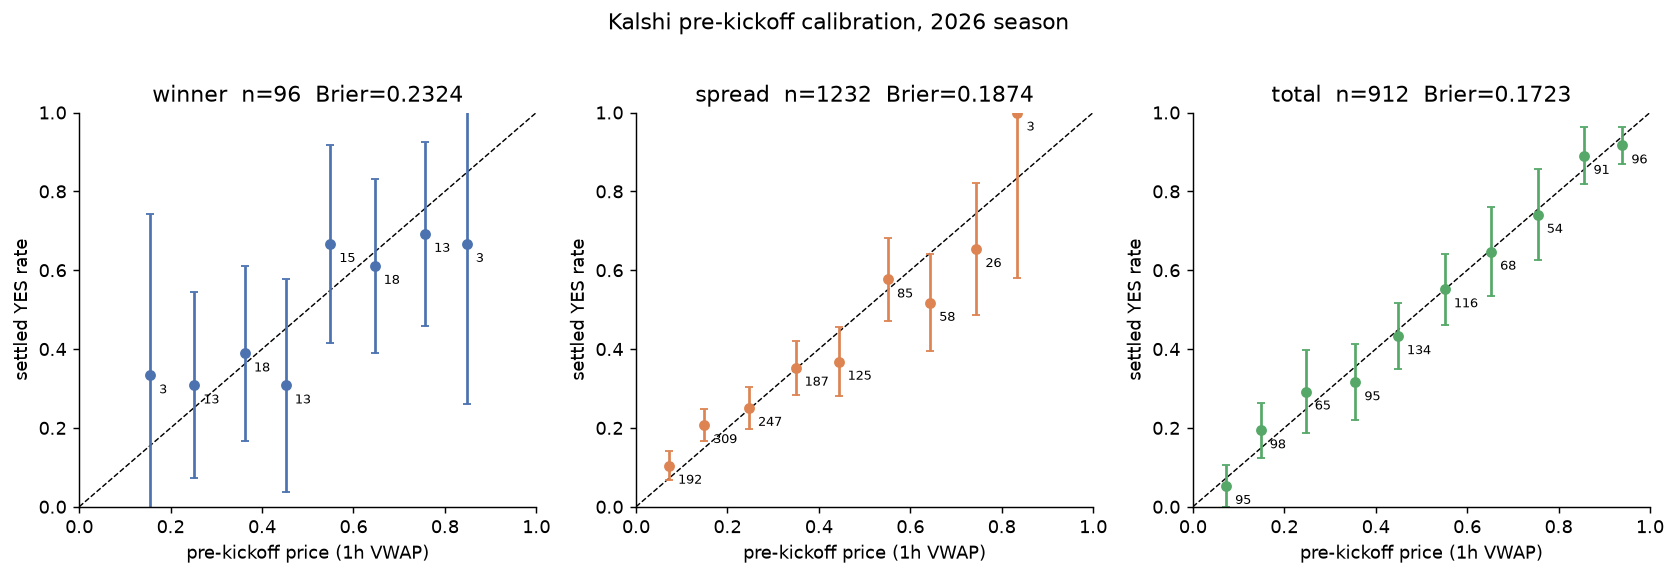
\includegraphics[width=0.95\textwidth]{kalshi_calibration.png}
\caption{Calibration of Kalshi pre-kickoff prices (1-hour volume-weighted average) against settlement, 2026 weeks 1--3, by contract type.}
\label{fig:kalshi_cal}
\end{figure}

\subsection{NFL results and the pre-game feature table}

Historical results, play-by-play, rosters, injury reports and closing lines come from the public nflverse project~\cite{nflverse}. From them we built a table of 7,548 games (1999--2026) with 805 columns, one row per game in home-team orientation (Table~\ref{tab:features}). All data is free.

\begin{table}[H]
\centering
\small
\begin{tabular}{p{2.2cm}rp{8.3cm}p{1.9cm}}
\toprule
\textbf{Group} & \textbf{Cols} & \textbf{Content} & \textbf{From} \\
\midrule
Team form & 604 & 20 offensive and 20 defensive efficiency statistics from play-by-play (EPA per play, success rate, pass and rush splits, explosive-play rate, yards per play, completion percentage over expected, turnovers, sacks, third-down rate, points per drive, neutral-script EPA), each over five windows (last 4, last 8, exponentially weighted, season to date, previous season), for home, away and the home-minus-away difference & 1999; CPOE 2006 \\
Ratings & 68 & Pre-game Elo (FiveThirtyEight recipe), exponentially weighted margin, opponent-adjusted margin & 1999 \\
Quarterback & 23 & Scheduled starter's weighted EPA per dropback, CPOE, sack and interception rates, career dropbacks, starter-change flag & 1999 \\
Injuries & 44 & Players Out/Doubtful and Questionable by position group; snap share of players now out & 2009; snaps 2013 \\
Situational & 31 & Rest, bye, short week, primetime, dome, surface, temperature, wind, divisional, playoff & 1999 \\
Market & 10 & Closing spread, total, moneylines; stored for benchmarking, never used as features & 1999 \\
Targets & 5 & Home score, away score, margin, total, home win & 1999 \\
\bottomrule
\end{tabular}
\caption{The pre-game feature table.}
\label{tab:features}
\end{table}

Every feature is computed from information dated before kickoff: rolling statistics are shifted by one game, Elo is the pre-update value, and injury counts come from the report filed before the game. Following Glickman and Stern~\cite{glickmanstern2017}, each team statistic enters as the home value, the away value and their difference. We test for leakage by perturbation: one game's play-level statistics are multiplied by ten and thirty points added to its score, the table is rebuilt, and the game's own 233 team features and Elo must be unchanged while the two teams' later games change. Six random games pass. The test earned its keep: the nflverse schedule carries two post-game fields, \texttt{result} and \texttt{total}, that equal the targets. A forest trained with them reported a margin error of 2.4 points with 85\% of its importance on those two columns; they were removed and the table re-scanned for any column correlated above 0.6 with a target.

{\color{red}\textbf{Amine comment:} Could you please state when forecasts are made and confirm that weather, starting-quarterback and injury information was available by then. Changing game statistics does not test when these other inputs became known.}

{\color{blue}\textbf{Sai comment:} Fixed. The paragraph below fixes the forecast time at kickoff and goes through each input: the starting quarterback is the recorded starter (known 90 minutes before kickoff), injuries come from the timestamped final report, and weather is the observed conditions; refitting without the weather columns changes the margin error by 0.001 points (Section~\ref{sec:scoremodel}).}

\paragraph{When the forecast is made.} The perturbation test checks that no feature uses the game's own plays or score; it does not check when each input became public. We fix the forecast time at kickoff, the same instant at which the closing line is taken, and list the inputs whose availability depends on that choice. \emph{Starting quarterback}: nflverse records the quarterback who started, which is the information a bettor has when the inactive list is published 90 minutes before kickoff; a forecast made earlier in the week would have to treat a doubtful starter as a probability. \emph{Injuries}: the counts come from the final official injury report, which nflverse timestamps (\texttt{date\_modified}); it is filed on the Friday or Saturday before a Sunday game, so it is available by kickoff and usually two days earlier. \emph{Weather}: the temperature and wind columns are the conditions recorded at the game, not a forecast, so they are strictly known only afterwards. A game-time forecast would be close but not identical. To bound what this costs, we refit the forest walk-forward with the four weather columns removed; the margin error changes by 0.001 points and the total error by 0.013 (Section~\ref{sec:scoremodel}). \emph{Rolling form, Elo, rest, venue} are known days in advance. No feature uses the betting line.

\subsection{Testing}

All programs are implemented in Python in a shared repository and run locally or on Google Colab. Models are evaluated walk-forward by season, training on all seasons before $t$ and testing on season $t$, because games within a season are related through the teams.

% ===== sections/week_0930.tex =====
\section{Weekly progress}\label{sec:weekly}

\subsection{Report of 30 September 2026: pricing as outcome modelling}\label{sec:w0930}

\textbf{Summary.} Framed pricing as outcome modelling (Section~\ref{sec:pricing}); surveyed the sports-pricing literature; pulled Kalshi markets, trades and candlesticks and nflverse results (Section~\ref{sec:data}); explored the empirical score distribution; built a worked example of an empirical distribution positioned to a game and priced against a live order book.



\subsubsection{What the empirical score distribution looks like}

Three findings from 3,076 games (2015--2026) constrain the shape of $p(h,a)$ (Figure~\ref{fig:keynumbers}). The absolute margin lands exactly on 3 in 14.8\% of games and on 7 in 8.7\%, 2.9 and 1.9 times what a normal distribution centred on the point spread implies; a smooth model misprices spread strikes near these ``key numbers'' by 5 to 10 cents. Margin and total are nearly uncorrelated (0.03) but share parity in every game, since they are the difference and sum of the same two integers, so half of the margin-by-total lattice is empty and a copula on the two marginals would put mass there. And the closing spread is an unbiased forecast with a residual standard deviation of 12.7 points, slightly tighter than the 13.86 of Stern~\cite{stern1991}.

\begin{figure}[H]
\centering
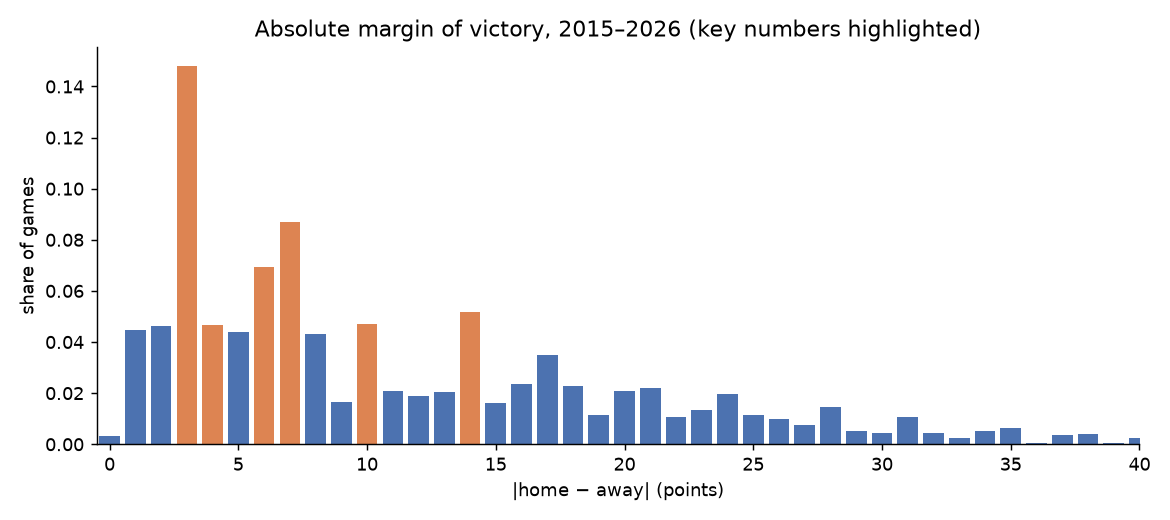
\includegraphics[width=0.95\textwidth]{nfl_abs_margin.png}
\caption{Absolute margin of victory, 2015--2026 (3,076 games); key numbers 3, 7, 6, 10 and 14 in orange.}
\label{fig:keynumbers}
\end{figure}

\begin{figure}[H]
\centering
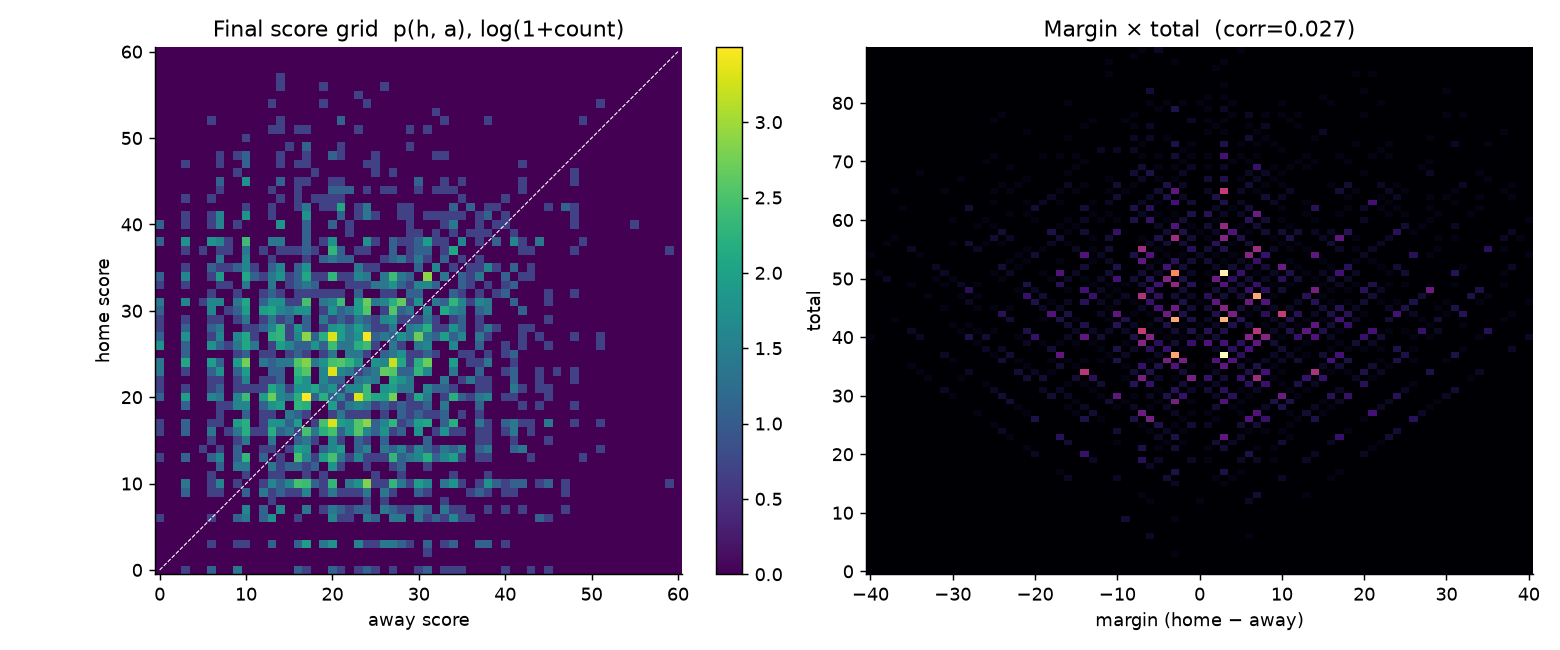
\includegraphics[width=0.95\textwidth]{nfl_score_grid.png}
\caption{Left: the empirical final-score grid $p(h,a)$ (log counts). Right: margin against total; the chequerboard is parity.}
\label{fig:scoregrid}
\end{figure}

\subsubsection{Positioning the empirical distribution for a game}

We want a distribution $p$ that (i) has the game's expected margin and total and (ii) is otherwise as close as possible to the historical prior $p_0$. Minimising the Kullback--Leibler divergence $\mathrm{KL}(p\,\|\,p_0)$ subject to the two moment constraints gives the exponential-family solution
\begin{equation}
p(h,a) \;\propto\; p_0(h,a)\,\exp\!\big(\lambda_1 (h-a) + \lambda_2 (h+a)\big),
\label{eq:tilt}
\end{equation}
with $(\lambda_1,\lambda_2)$ solved so that $\mathbb{E}[h-a]$ and $\mathbb{E}[h+a]$ match the targets, a two-equation root find. Because the tilt only reweights cells, it cannot create mass where the prior has none: a 3-point win stays 2.9 times as likely as a 4-point win. A Poisson or normal model would have to be taught key numbers, parity and cell clustering; the empirical grid already has them.

{\color{red}\textbf{Amine comment:} Could a possible score pair receive zero probability simply because it is absent from the historical sample? How such outcomes are handled and how smoothing affects extreme-outcome probabilities and expected shortfall.}

{\color{blue}\textbf{Sai comment:} Fixed. The paragraph and Table~\ref{tab:smoothing} below quantify it: 19--31\% of a season's games land on an unseen exact pair, the 2\% pseudo-count fills every cell whose two scores have been seen, and moving it from 0 to 10\% shifts tail probabilities by hundredths of a point and a deep strike's ES$_{99}$ by under 0.5\%.}

\paragraph{Score pairs never seen.} The reweighting property cuts both ways: a reachable score pair that is absent from the sample would keep probability zero under any tilt. This is not rare. Of the roughly 6,400 reachable cells (either score $0$--$80$ except $1$), the 3,028 games of 2015--2025 occupy 1,065, and between 19\% and 31\% of a season's games end on an exact pair that had not occurred in the preceding seasons since 2015 (31\% in 2020, 19\% in 2023, 22\% in 2025). We therefore add a pseudo-count: a mass of 2\% spread over the cells in proportion to the product of the two marginal score distributions, which fills every cell whose two scores have each been seen (2,850 cells) and leaves at zero only combinations involving a score never recorded. The exact pair matters for a log-likelihood but not for a contract, since every contract is a sum over a region of the grid and the regions near the tails contain many cells. Table~\ref{tab:smoothing} shows the effect of the pseudo-count on the tilted grid of a typical line: tail probabilities move by a few hundredths of a percentage point and the 99\% expected shortfall of a deep strike by less than 0.5\%. The choice of 2\% is a convention; moving it to 10\% changes the same quantities by about one part in fifty, with the largest effect on the price of the deepest strikes, which is where the sample is thinnest and a model-based tail would be the better tool.

\begin{table}[H]
\centering
\small
\begin{tabular}{lccc}
\toprule
\textbf{Pseudo-count mass} & \textbf{0} & \textbf{2\% (used)} & \textbf{10\%} \\
\midrule
Non-zero cells & 1,065 & 2,850 & 2,850 \\
$P(|h-a|\ge 21)$ & 16.53\% & 16.51\% & 16.42\% \\
$P(|h-a|\ge 28)$ & 6.86\% & 6.83\% & 6.72\% \\
$P(|h-a|\ge 42)$ & 0.345\% & 0.344\% & 0.340\% \\
$P(h+a\ge 70)$ & 4.07\% & 4.06\% & 4.05\% \\
Price of ``home wins by $>27.5$'' & 1.95\textcent & 1.94\textcent & 1.90\textcent \\
ES$_{99}$, short 1,000 of that contract & \$980.5 & \$980.6 & \$981.0 \\
ES$_{99}$, short 1,000 of ``over 69.5'' & \$959.3 & \$959.4 & \$959.5 \\
\bottomrule
\end{tabular}
\caption{Effect of the pseudo-count on the 2015--2025 grid tilted to home $-3$, total 44.5.}
\label{tab:smoothing}
\end{table}

\subsubsection{Worked example: Pittsburgh at Cleveland} Pittsburgh at Cleveland, 1 October 2026, with the live Kalshi order book captured the day before (46 contracts). The sportsbook line was Cleveland $-2.5$ and total 38.5. Tilting the 3,076-game prior to those two numbers gives $\lambda_1=-0.0222$, $\lambda_2=-0.0399$ (Figures~\ref{fig:toy_dist} and~\ref{fig:toy_grid}). Table~\ref{tab:toy} compares model prices with the Kalshi mid for every contract.

\begin{figure}[H]
\centering
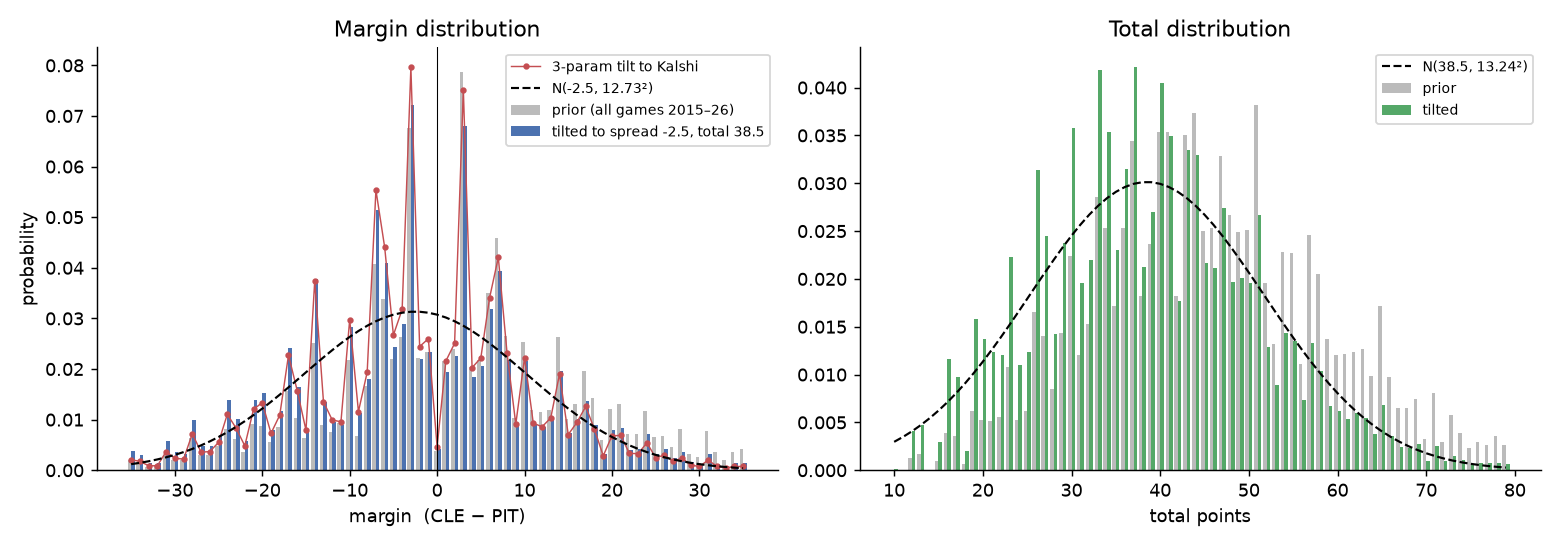
\includegraphics[width=0.98\textwidth]{toy_margin_total.png}
\caption{Margin (left) and total (right) distributions: grey the prior, blue the prior tilted to the book line, red a three-parameter tilt calibrated to Kalshi, dashed the normal.}
\label{fig:toy_dist}
\end{figure}

\begin{figure}[H]
\centering
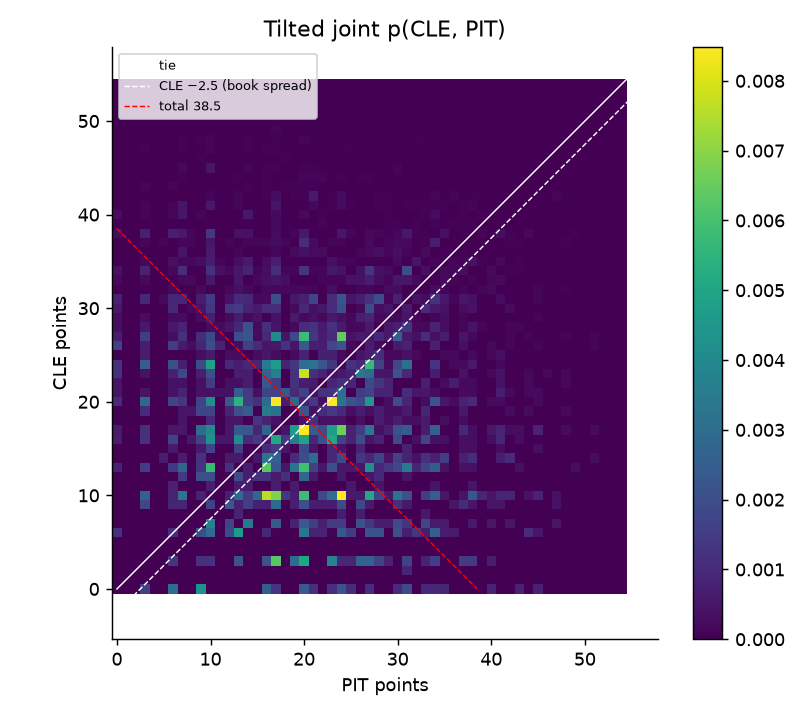
\includegraphics[width=0.6\textwidth]{toy_joint_grid.png}
\caption{The tilted joint table for Pittsburgh at Cleveland. The diagonal is a tie, the dashed line the book spread and the red line the total; each contract is a sum over one side of one of these lines.}
\label{fig:toy_grid}
\end{figure}

\begin{table}[H]
\centering
\footnotesize
\begin{tabular}{lcccc}
\toprule
\textbf{Model} & \textbf{All 46} & \textbf{Winner} & \textbf{Spread strikes} & \textbf{Total strikes} \\
\midrule
Untilted prior & 11.2 & 12.5 & 8.7 & 14.3 \\
Normal around the line & 1.89 & 0.28 & 2.32 & 1.48 \\
Tilt to the book line (no Kalshi data) & 1.52 & 0.08 & 1.98 & 1.06 \\
Two-parameter tilt fitted to Kalshi mids & 1.49 & 0.76 & 2.00 & 0.88 \\
Three-parameter tilt (adds margin$^2$) fitted to Kalshi & 0.76 & 0.24 & 0.64 & 0.99 \\
\bottomrule
\end{tabular}
\caption{Mean absolute error in cents of model price against the Kalshi mid, Pittsburgh at Cleveland. Quoted bid--ask spreads were 1--2 cents.}
\label{tab:toy}
\end{table}

\begin{figure}[H]
\centering
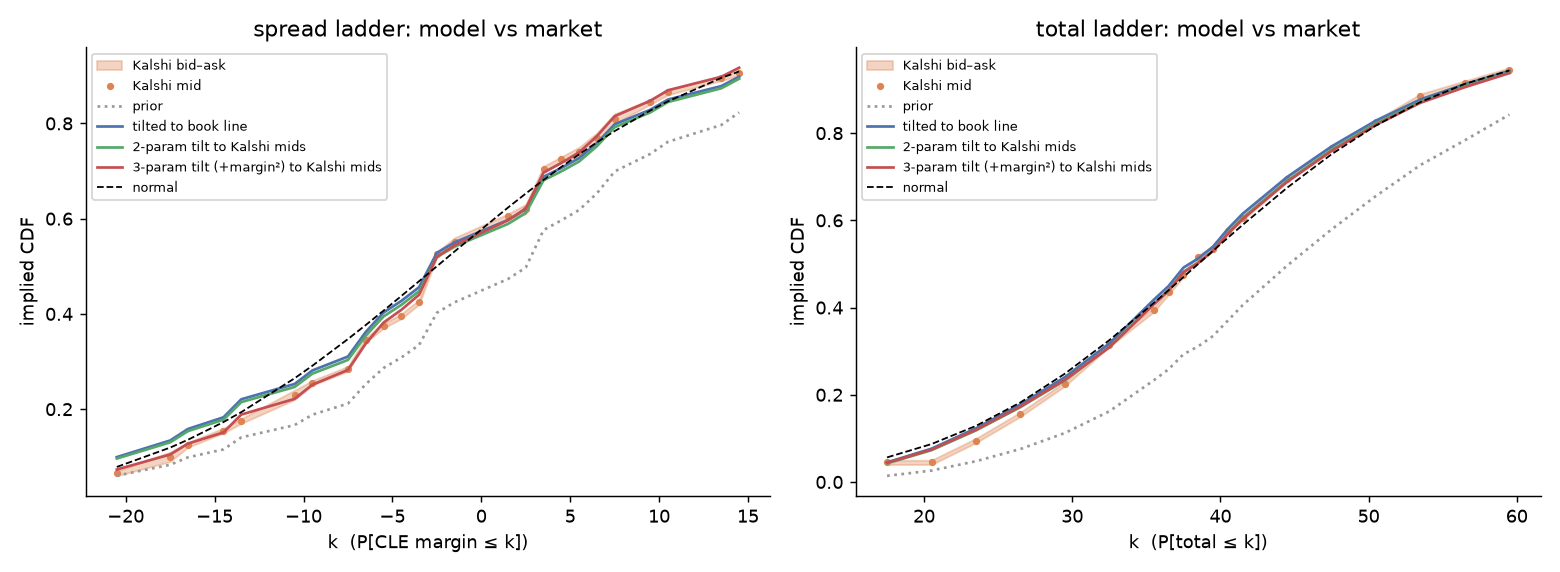
\includegraphics[width=0.98\textwidth]{toy_ladders.png}
\caption{Market-implied cumulative distributions from the spread (left) and total (right) ladders against the model variants. The shaded band is the Kalshi bid--ask.}
\label{fig:toy_ladders}
\end{figure}

Three lessons follow. Locating the distribution with the book line removes 87\% of the pricing error and prices the winner contract to 0.1 cents. Discreteness matters on the ladder: the normal is off by up to 6 cents on a single strike. And two moments do not control the tails: the book-tilted grid overprices Pittsburgh blowouts by 2--4.5 cents because the prior's margin has standard deviation 14.2 while the market prices this low-scoring game nearer 12.3. A third parameter on $(h-a)^2$ lets the market set the dispersion and the tail error disappears. This is the strongest argument for a model that predicts dispersion as well as location, and it motivates the score model of Section~\ref{sec:scoremodel}.

\subsubsection{What moves a game's expected score}

Before building features we listed the factors practitioners weigh when setting a line (Table~\ref{tab:factors}); the feature table of Section~\ref{sec:data} covers all but travel distance.

\begin{table}[H]
\centering
\small
\begin{tabular}{p{3cm}p{2.4cm}p{8.4cm}}
\toprule
\textbf{Factor} & \textbf{Typical effect} & \textbf{Notes} \\
\midrule
Starting quarterback & $\pm$3 to 10 pts & The largest single factor; elite starter versus backup is worth 7--10 points or 20--25 percentage points of win probability. Status should be modelled as a probability when questionable. \\
Team strength & baseline & Elo or power ratings, or EPA per play and success rate on offence and defence; adjust for opponent and regress toward the mean early in the season. \\
Home field & 1.5 to 2 pts & Has shrunk over the past decade; varies by venue and travel. \\
Other key injuries & 0.5 to 2 pts each & Costliest at offensive tackle, edge rusher, top cornerback and top receiver; multiple injuries on one unit compound. \\
Rest and schedule & 0.5 to 1.5 pts & Bye week helps; short week and long road trips hurt; time-zone changes matter for early-kickoff West Coast teams. \\
Weather and venue & totals & Wind above 15 mph and heavy precipitation suppress scoring; lowers the total and compresses variance. Domes remove it. \\
Coaching & 0.5 to 1 pt & Fourth-down aggressiveness, clock management, in-game adjustments. \\
Motivation and context & small, noisy & Playoff seeding, eliminated teams and week-18 rest can matter in specific spots. \\
Turnover luck & shrinkage & Fumble recoveries and close-game records are largely noise; use them to shrink apparent strength. \\
\bottomrule
\end{tabular}
\caption{Factors in a game's expected score, with typical magnitudes as cited by practitioners.}
\label{tab:factors}
\end{table}

\textbf{Conclusion of the week.} It is better to build the scoring model first: predict the two absolute scores, home and away, from pre-game features, and let the score grid turn them into prices. Professors Amine and Shasha suggested dimensionality reduction (PCA, UMAP), a multi-output random forest, LARS and cascade-correlation networks, a multi-output linear baseline, and a neural network parameterising a bivariate Gaussian $(\mu_h,\mu_a,\sigma_h,\sigma_a,\rho)$; Professor Shasha noted that random forests, especially with boosting, handle many features without reduction and discard what is useless.

% ===== sections/week_1007.tex =====
\subsection{Report of 7 October 2026: literature, feature table, two-output random forest}\label{sec:w1007}

\textbf{Summary.} The question after the first report was whether anyone has predicted NFL scores before, with what data, and how. This week: a literature survey; a catalogue of the data used in the literature against what nflverse provides; the 805-column pre-game feature table with its leakage test (Section~\ref{sec:data}); and a first two-output random forest evaluated walk-forward over sixteen seasons.

\subsubsection{Literature}\label{sec:literature}


The first question raised after the 30 September report was whether anyone has tried to predict NFL scores before, what data they used, and how they thought about the problem. The literature falls into five groups.

\paragraph{Rating models from scores alone.} Harville~\cite{harville1980} fitted a mixed linear model to score differences from 1,320 games and obtained an average error of 10.68 points against 10.49 for the bookmaker. Glickman and Stern~\cite{glickmanstern1998} let each team's strength drift from week to week and season to season in a Bayesian state-space model and matched the Las Vegas line on a 1993 test set. Their handbook chapter~\cite{glickmanstern2017} surveys these methods and recommends entering each covariate as the difference and the average of the two teams' values, which we adopted. FiveThirtyEight's Elo system~\cite{fivethirtyeightelo} is the practical version: one strength number per team updated from margin of victory, with adjustments for home field, rest and the starting quarterback. All of these use only results and the schedule, and all land a few tenths of a point behind the line.

\paragraph{Exact scores and distributions.} Baker and McHale~\cite{bakermchale2013} is the only paper that forecasts both teams' exact NFL scores, with a birth-process model and pre-game covariates; it too performs about as well as the bookmaker. Stern~\cite{stern1991} showed that margin minus spread is approximately normal with standard deviation near 14, which gives the standard conversion from a spread to a win probability; Stern~\cite{stern1994} and Polson and Stern~\cite{polsonstern2015} extend this to the progress of a game and to a market-implied volatility. In soccer, Dixon and Coles~\cite{dixoncoles1997} model scores as correlated Poisson counts and Divos et al.~\cite{divos2018} price in-play bets by risk-neutral methods; the lesson for us is that football scoring is discrete in a way Poisson models do not capture.

\paragraph{Play-level information.} Yurko, Ventura and Horowitz~\cite{yurko2019} defined expected points and win probability from play-by-play data and showed how to attribute them to plays and players. Expected points added per play is the efficiency measure the analytics community has settled on; the nflverse project provides it for every play since 1999 and it is the source of most of our team-form features.

\paragraph{Market efficiency.} Levitt~\cite{levitt2004} showed from a bettor-level dataset that bookmakers do not balance their books but set prices as skilled forecasts that exploit bettor biases, which is why the closing line is hard to beat. Boulier and Stekler~\cite{boulierstekler2003} and Song, Boulier and Stekler~\cite{songboulierstekler2007} compared statistical systems, experts and the betting market and found the market most accurate, with models and experts tied. Zuber, Gandar and Bowers~\cite{zuber1985} and Gray and Gray~\cite{graygray1997} found only small, unstable inefficiencies. Lopez, Matthews and Baumer~\cite{lopez2018} go the other way and use moneylines as the best available measure of team strength. Shin~\cite{shin1993} and Wolfers and Zitzewitz~\cite{wolferszitzewitz2006} show how to read probabilities from odds and from prediction-market prices.

\paragraph{Machine-learning studies.} A systematic review by Galekwa et al.~\cite{mlreview2024} and a number of student projects report accuracies of 70 to 95 percent at picking winners. Where the methods are described, these come from same-game statistics (leakage) or from very small test sets. The closing line picks the winner about 66 percent of the time; nothing credible is far above that. We took two lessons: build an explicit leakage test, and do not expect a flexible learner to add much over a well-specified rating model with 7,000 games.

\paragraph{Data in the literature.} The serious score models use only scores, dates and home field; richer inputs appear in three families: play-level efficiency, quarterback identity and betting lines. Bet-volume data (Levitt; Paul and Weinbach) is proprietary; the Kalshi trade tape is the free equivalent. No paper reviewed uses injuries, snap counts or depth charts in a score model, although Glickman and Stern~\cite{glickmanstern2017} name player-level factors as the obvious gap. Everything the literature uses is available free from nflverse except opening lines and bet splits.

\paragraph{Implication for our design.} Point accuracy for NFL scores is capped near the closing line for every published method. The sensible goal is a calibrated distribution over both scores, consistent across every derived quantity, rather than a lower point error. The suggestions received from Professors Amine and Shasha fit this picture: a multi-output random forest can use every feature without selection, a linear baseline shows whether the forest adds anything, and a probabilistic extension predicting two means, two standard deviations and a correlation is the natural destination for a two-score model.

\subsubsection{Predicting both teams' scores}\label{sec:scoremodel}


\paragraph{Why two scores.}

The object the engine needs is the joint distribution over $(h,a)$. Predicting each team's score is the natural first step: the two predictions locate the centre of that distribution and the spread of the residuals around them gives its width. A model for the margin alone discards the level of scoring; a 30--27 game and a 17--14 game have the same margin and very different distributions of totals and of every strike.

\paragraph{Models and evaluation.}

Table~\ref{tab:models} lists the models. All use the 759 non-market features of Section~\ref{sec:data}; the closing line is a benchmark only. Evaluation is walk-forward: train on every season before $t$, test on season $t$, for $t = 2010,\dots,2025$ (4,363 test games).

\begin{table}[H]
\centering
\small
\begin{tabular}{p{3.6cm}p{6.2cm}p{4cm}}
\toprule
\textbf{Model} & \textbf{Inputs} & \textbf{Role} \\
\midrule
League average & Mean scores in the training seasons & Floor \\
Elo & Results only; implied spread is Elo difference / 25 & Rating baseline \\
Two-output ridge regression & 759 features, median-imputed, standardised, penalty by cross-validation & Linear baseline \\
Two-output random forest & 759 features, 500 trees, at least 20 games per leaf, 30\% of features per split, no tuning & Main model: predicts $(h,a)$ jointly \\
Closing line & Consensus sportsbook spread and total & Benchmark \\
\bottomrule
\end{tabular}
\caption{Models compared. The forest predicts the two scores as a pair: each leaf holds the mean home and away score of similar past games.}
\label{tab:models}
\end{table}

\paragraph{Point accuracy.}

\begin{table}[H]
\centering
\small
\begin{tabular}{lcccc}
\toprule
\textbf{Model} & \textbf{Home score} & \textbf{Away score} & \textbf{Margin} & \textbf{Total} \\
\midrule
League average & 8.09 & 7.91 & 11.18 & 11.02 \\
Elo & -- & -- & 10.38 & -- \\
Two-output ridge & 7.62 & 7.40 & 10.34 & 10.63 \\
Two-output random forest & 7.63 & 7.45 & 10.35 & 10.66 \\
Closing line & -- & -- & \textbf{10.05} & \textbf{10.47} \\
\bottomrule
\end{tabular}
\caption{Mean absolute error in points, walk-forward 2010--2025.}
\label{tab:mae}
\end{table}

The forest explains 10.8\% of the variance of the home score and 9.3\% of the away score out of sample. These numbers are normal for the problem: a single game is mostly noise around a modest signal, and the closing line, with every input a bettor can find, explains only a little more. The forest and the ridge are indistinguishable at every target. On the margin they are 0.03--0.04 points better than Elo and 0.3 points worse than the line (Figure~\ref{fig:mae_season}); the line has the lowest error in 15 of 16 seasons. Straight-up winner accuracy is 64.7\% for the forest, 64.6\% for ridge, 64.5\% for Elo and 66.3\% for the line. Against the spread the forest picks the covering side 49.9\% of the time, as an efficient line implies.

{\color{red}\textbf{Amine comment:} Please report uncertainty for the differences in error on the same games, allowing for dependence over time, and clarify forecast timing relative to the closing line. The table shows gains over Elo of 0.03--0.04 points, not a quarter point.}

{\color{blue}\textbf{Sai comment:} Fixed. The ``quarter of a point'' is corrected to 0.03--0.04 above; the paragraph and Table~\ref{tab:mae_diff} below give paired error differences with i.i.d., week-clustered, season-clustered and Newey--West standard errors (gain over Elo about one standard error; gap to the line seven to eight), and state that model and line are both taken at kickoff.}

Because every forecast is scored on the same 4,363 games, the differences between them are paired, and their uncertainty has to allow for the fact that games in the same week and season are related. Table~\ref{tab:mae_diff} gives the mean difference in absolute margin error for each pair with four standard errors: treating games as independent, clustering by week (271 clusters), clustering by season (16 clusters), and a Newey--West estimate over the game sequence with a lag of four weeks. The four agree closely, which says the game-level errors are nearly uncorrelated once the forecasts are differenced. The gain over Elo, $0.03$--$0.04$ points, is about one standard error and shows up in only 9 or 10 of the 16 seasons: it is not distinguishable from zero. The gap to the closing line, $0.29$--$0.33$ points, is seven to eight standard errors and holds in 15 of 16 seasons. The forest and the ridge differ by $0.01 \pm 0.03$. On timing, every model forecast uses only information available at kickoff and none uses the line (Section~\ref{sec:data}); the closing line is also the kickoff price, so the two are compared at the same instant. The weather columns are the one input strictly observed rather than forecast. Refitting the forest walk-forward without the four weather columns (\texttt{scripts/model\_rf\_noweather.py}) changes the margin error from 10.352 to 10.353 and the total error from 10.663 to 10.676, so nothing in the comparison rests on knowing the weather in advance.

\begin{table}[H]
\centering
\footnotesize
\setlength{\tabcolsep}{4pt}
\begin{tabular}{lrrrrrrc}
\toprule
\textbf{Difference in MAE} & \textbf{Mean} & \textbf{SE i.i.d.} & \textbf{SE week} & \textbf{SE season} & \textbf{SE NW} & \textbf{$t$, 16 seasons} & \textbf{Seasons better} \\
\midrule
Forest $-$ Elo & $-0.030$ & 0.029 & 0.028 & 0.032 & 0.029 & $-0.9$ & 10 of 16 \\
Ridge $-$ Elo & $-0.041$ & 0.039 & 0.040 & 0.034 & 0.036 & $-1.2$ & 9 of 16 \\
Forest $-$ Ridge & $+0.011$ & 0.029 & 0.031 & 0.022 & 0.028 & $0.5$ & 6 of 16 \\
Forest $-$ Line & $+0.298$ & 0.043 & 0.041 & 0.039 & 0.040 & $7.5$ & 1 of 16 \\
Ridge $-$ Line & $+0.287$ & 0.043 & 0.042 & 0.038 & 0.040 & $7.4$ & 1 of 16 \\
Elo $-$ Line & $+0.328$ & 0.045 & 0.045 & 0.040 & 0.042 & $8.0$ & 1 of 16 \\
\bottomrule
\end{tabular}
\caption{Paired differences in absolute margin error, 4,363 games, 2010--2025. Negative means the first forecast is better. The $t$ statistic is the season-level paired $t$ on the 16 seasonal means; the last column counts seasons in which the first forecast had the lower error.}
\label{tab:mae_diff}
\end{table}

\begin{figure}[H]
\centering
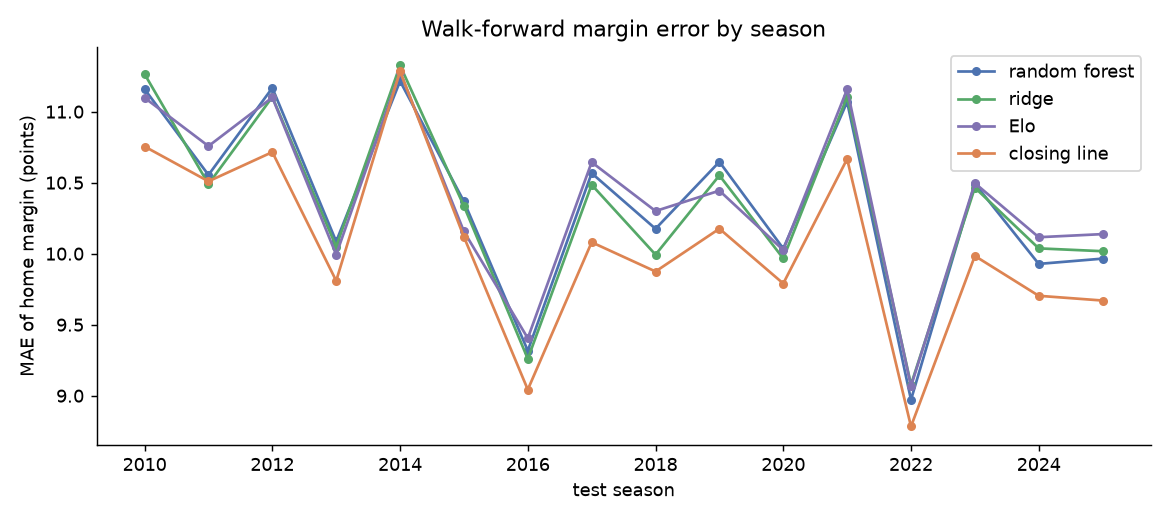
\includegraphics[width=0.95\textwidth]{rf_mae_by_season.png}
\caption{Margin error by test season. All methods share the hard and easy seasons; the closing line is lowest in 15 of 16.}
\label{fig:mae_season}
\end{figure}

\begin{figure}[H]
\centering
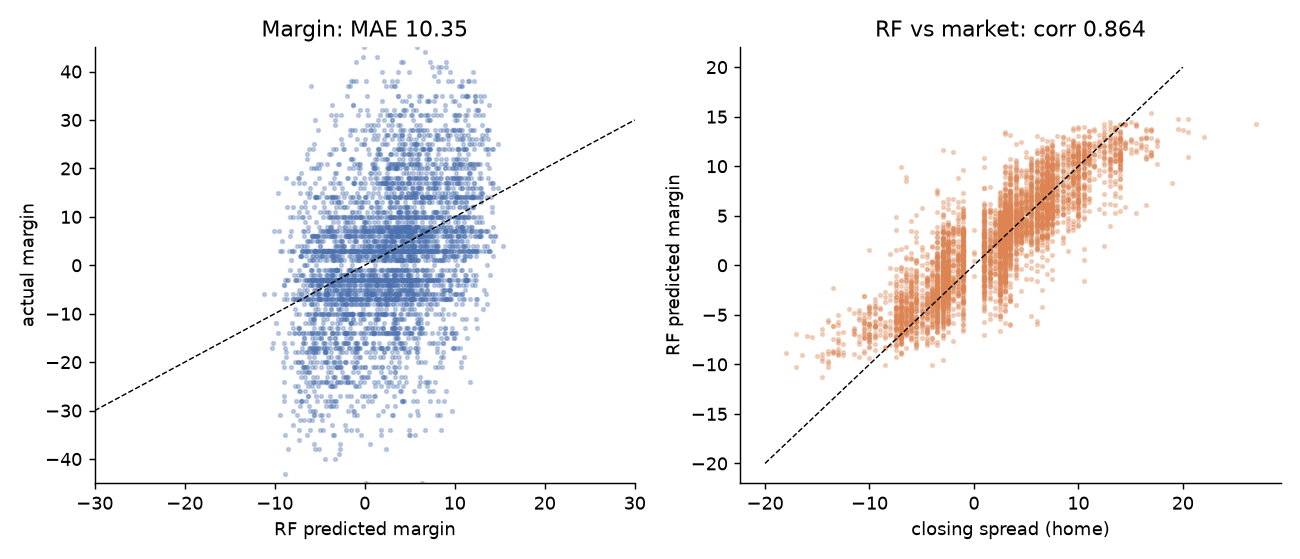
\includegraphics[width=0.95\textwidth]{rf_pred_vs_actual.png}
\caption{Left: predicted against actual margin. Right: the forest's margin against the closing spread (correlation 0.86).}
\label{fig:pred_actual}
\end{figure}

\paragraph{The two-output structure.}

Because the forest predicts a point in the $(h,a)$ plane, its residuals describe a two-dimensional distribution around that point (Table~\ref{tab:bivariate}, Figure~\ref{fig:bivariate}). The correlation between the home and away residuals is 0.01: once the two means are set, the leftover error in one score says nothing about the other. Residual spread grows with the predicted score, so high-scoring games are less predictable in points, as a Poisson-like scoring process implies. Calibration per score is good: when the forest predicts 20 points the team scores 20 on average, across the range 15 to 33.

\begin{table}[H]
\centering
\small
\begin{tabular}{lcc}
\toprule
\textbf{Quantity} & \textbf{Home} & \textbf{Away} \\
\midrule
Standard deviation of the actual score & 10.21 & 9.83 \\
Standard deviation of the residual & 9.64 & 9.36 \\
Range of predicted scores & 15.8 to 33.3 & 13.3 to 30.4 \\
Residual s.d., lowest third of predictions & 9.20 & 8.88 \\
Residual s.d., highest third of predictions & 10.11 & 9.76 \\
\bottomrule
\end{tabular}
\caption{Residual structure of the two-output forest, 4,363 out-of-sample games. Residual correlation 0.011.}
\label{tab:bivariate}
\end{table}

\begin{figure}[H]
\centering
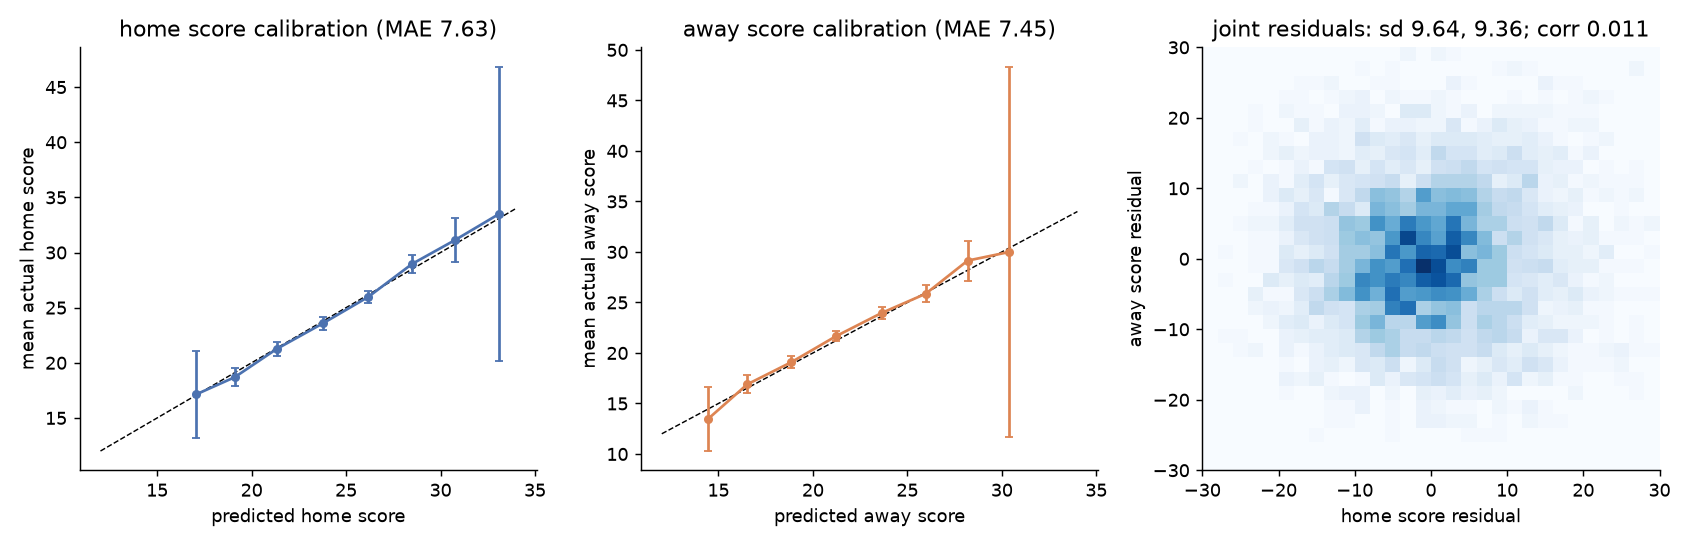
\includegraphics[width=0.98\textwidth]{rf_bivariate.png}
\caption{Calibration of the home and away score predictions and the joint distribution of the two residuals.}
\label{fig:bivariate}
\end{figure}

These residual statistics are the parameters $(\sigma_h,\sigma_a,\rho)$ of the probabilistic extension suggested by Professor Amine. Table~\ref{tab:bivariate} and Figure~\ref{fig:bivariate} pool the residuals of all sixteen test seasons, which is the right thing for describing them but not for scoring probabilities on those same seasons. For scoring we refit them walk-forward: the probability for a game in season $t$ uses the residual standard deviations and correlation of the out-of-sample predictions for seasons $2010$ to $t-1$ only, so the first scored season, 2016, uses six seasons of residuals (1,602 games) and 2025 uses fifteen (4,078). The margin standard deviation estimated this way runs from 13.87 (for 2016) down to 13.40 (for 2025), against 13.36 pooled. Used as a bivariate normal around the two predicted scores, the fold-wise residuals give a home-win probability with Brier score 0.2208 over 2016--2025 (0.2207 with the pooled values), against 0.2220 for Elo and 0.2108 for the de-vigged moneyline. The empirical grid used for the alternative, placing the two predicted means on the score table of Section~\ref{sec:pricing}, was already fold-wise: its prior for season $t$ is the table of all games before $t$, and it gives 0.2213. The probabilities are calibrated (Figure~\ref{fig:rf_cal}); the gap to the market is in sharpness, not bias.

{\color{red}\textbf{Amine comment:} Please confirm that residual covariance and the empirical grid use only earlier games in each test fold. Their stated estimation periods overlap the evaluation years.}

{\color{blue}\textbf{Sai comment:} Fixed. The grid prior was already fold-wise (all games before the test season). The residual covariance was pooled; it is now refit walk-forward from seasons before each test season, as the paragraph above reports (Brier 0.2208 fold-wise against 0.2207 pooled), and the pooled table and figure are labelled as descriptive.}

\begin{figure}[H]
\centering
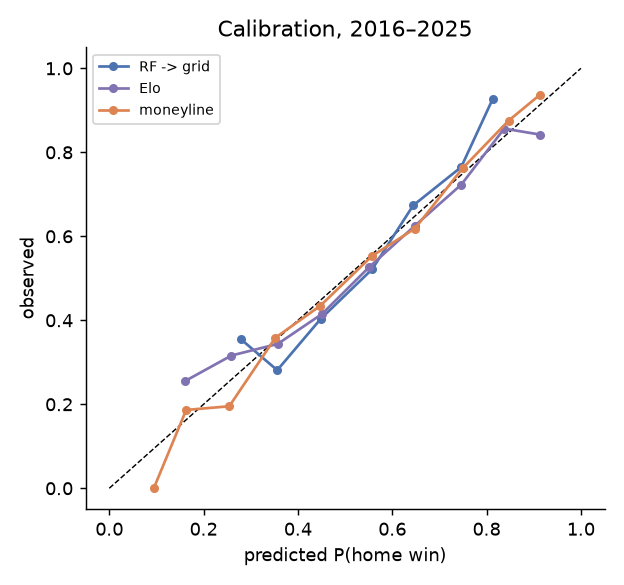
\includegraphics[width=0.5\textwidth]{rf_calibration.png}
\caption{Calibration of home-win probabilities, 2016--2025.}
\label{fig:rf_cal}
\end{figure}

\paragraph{What the forest uses.}

Averaged over the sixteen fits, the five most important features are all team-strength summaries from results: the difference in opponent-adjusted weighted margin, the difference in weighted margin, and the three Elo features (Figure~\ref{fig:importance}). The first play-by-play feature is yards per play, followed by the starting quarterback's success rate and EPA per dropback and points per drive. Injury, rest and weather features are far down the list. Most of what the model knows is how good each team has been; the efficiency and quarterback features refine that at the margin. The forest used all 759 features with no selection or tuning and matched a regularised linear model, which is what Professor Shasha expected.

\begin{figure}[H]
\centering
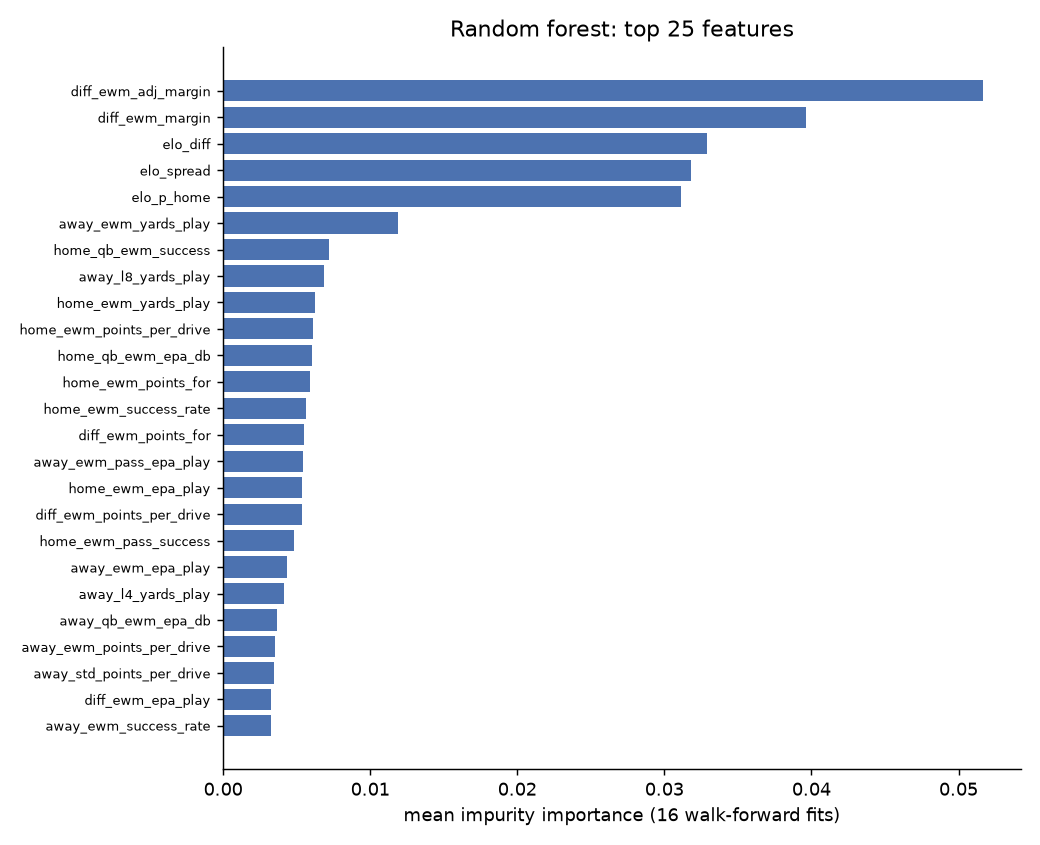
\includegraphics[width=0.75\textwidth]{rf_importance.png}
\caption{Top 25 features by mean impurity importance over the sixteen walk-forward fits.}
\label{fig:importance}
\end{figure}


% ===== sections/week_1021.tex =====
\subsection{Report of 21 October 2026: ensembles and full distributions}\label{sec:w1021}

\textbf{Summary.} Two questions from Professor Shasha: can an ensemble of the models we have, or can obtain, do better; and can the models give a distribution for the margin and the total, compared with the Vegas lines.

\subsubsection{Can an ensemble do better?}

Professor Shasha asked whether an ensemble of the models we have, or can obtain, improves on them. We stacked by least squares, fitting weights on earlier seasons' out-of-sample predictions and applying them to the next season, 2013--2025. To our three models we added two public forecasts, nfelo~\cite{nfelo} (a public Elo variant with a quarterback adjustment; we use its rating difference before any regression toward the market) and FiveThirtyEight's Elo (available to 2020), and the sportsbook \emph{opening} line, which the nfelo files carry (Table~\ref{tab:ensemble}, Figure~\ref{fig:ensemble}).

\begin{table}[H]
\centering
\small
\begin{tabular}{lcp{6cm}}
\toprule
\textbf{Forecast} & \textbf{Margin MAE} & \textbf{Note} \\
\midrule
Random forest (ours) & 10.22 & \\
Ridge (ours) & 10.20 & \\
Elo (ours) & 10.25 & \\
Stack of our three & 10.18 & weights 0.19 / 0.36 / 0.51 \\
nfelo, pure model & 10.01 & history back-computed with the current model, so optimistic \\
Stack: ours + nfelo & 10.04 & our models receive weight near 0 \\
Opening line & 10.02 & \\
Closing line & 9.92 & \\
Stack: ours + nfelo + closing line & 9.95 & closing line 0.58, nfelo 0.72, ours near 0 \\
\bottomrule
\end{tabular}
\caption{Stacking test, home margin, 2013--2025 (3,562 games with all forecasts available).}
\label{tab:ensemble}
\end{table}

\begin{figure}[H]
\centering
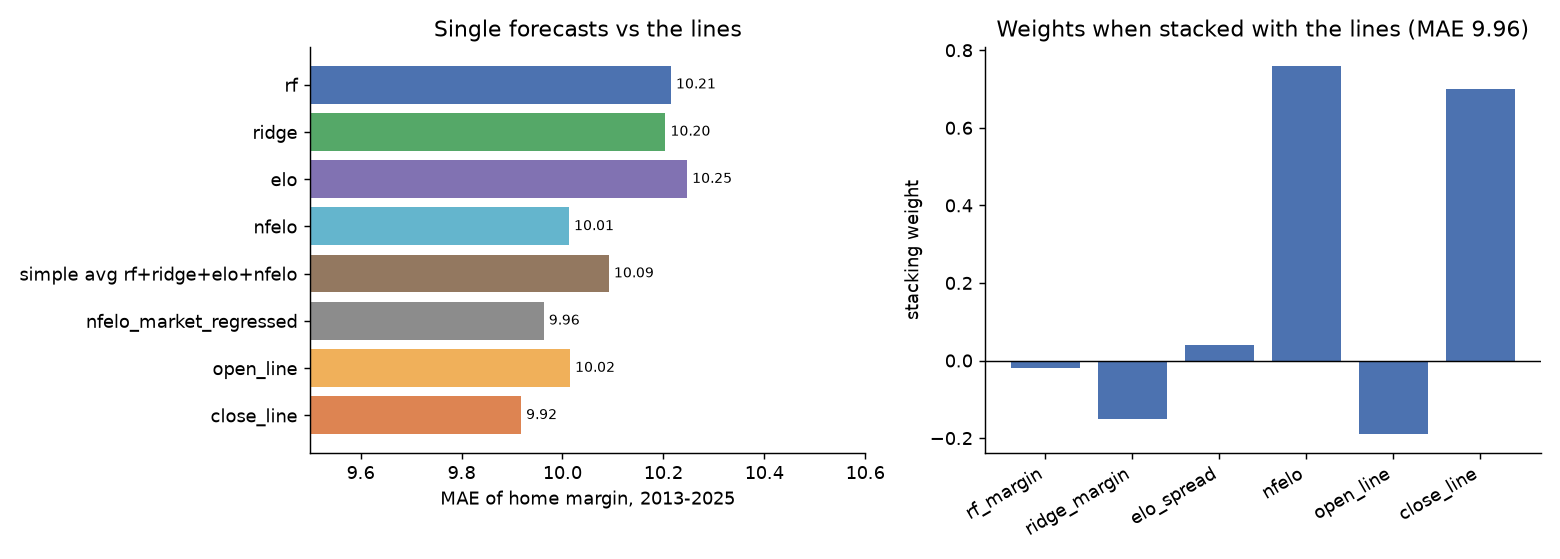
\includegraphics[width=0.98\textwidth]{ensemble_external.png}
\caption{Left: single forecasts and the lines. Right: stacking weights when our models, nfelo and both lines are combined.}
\label{fig:ensemble}
\end{figure}

Averaging our own models gains only a few hundredths of a point, because their predictions are correlated at 0.89--0.94. nfelo is a better single forecast than anything we built, by about 0.2 points, which we attribute to its quarterback adjustment and to its published history being generated by the current version of the model. Most important, no stack improves on the closing line: whenever the line is a component it takes nearly all the weight. The same holds for totals, where the opening total (10.47) is in fact slightly better than the closing total (10.53) in this sample. Ensembling what we have does not beat the market; an ensemble that could would need forecasts carrying information the market does not yet have.

\subsubsection{Full distributions and the Vegas lines}

The second question was whether the models can give a distribution for the margin and the total and how it compares with the lines. The two predicted scores set the centre, and the distribution around them comes either from the bivariate normal with the residual covariance or from the empirical grid tilted so that its mean margin and total match the forest (Figure~\ref{fig:gamedist}). From either, the probability of any outcome is a sum: $P(\text{home wins})$, $P(\text{home covers the spread})$, $P(\text{over the total})$.

\begin{figure}[H]
\centering
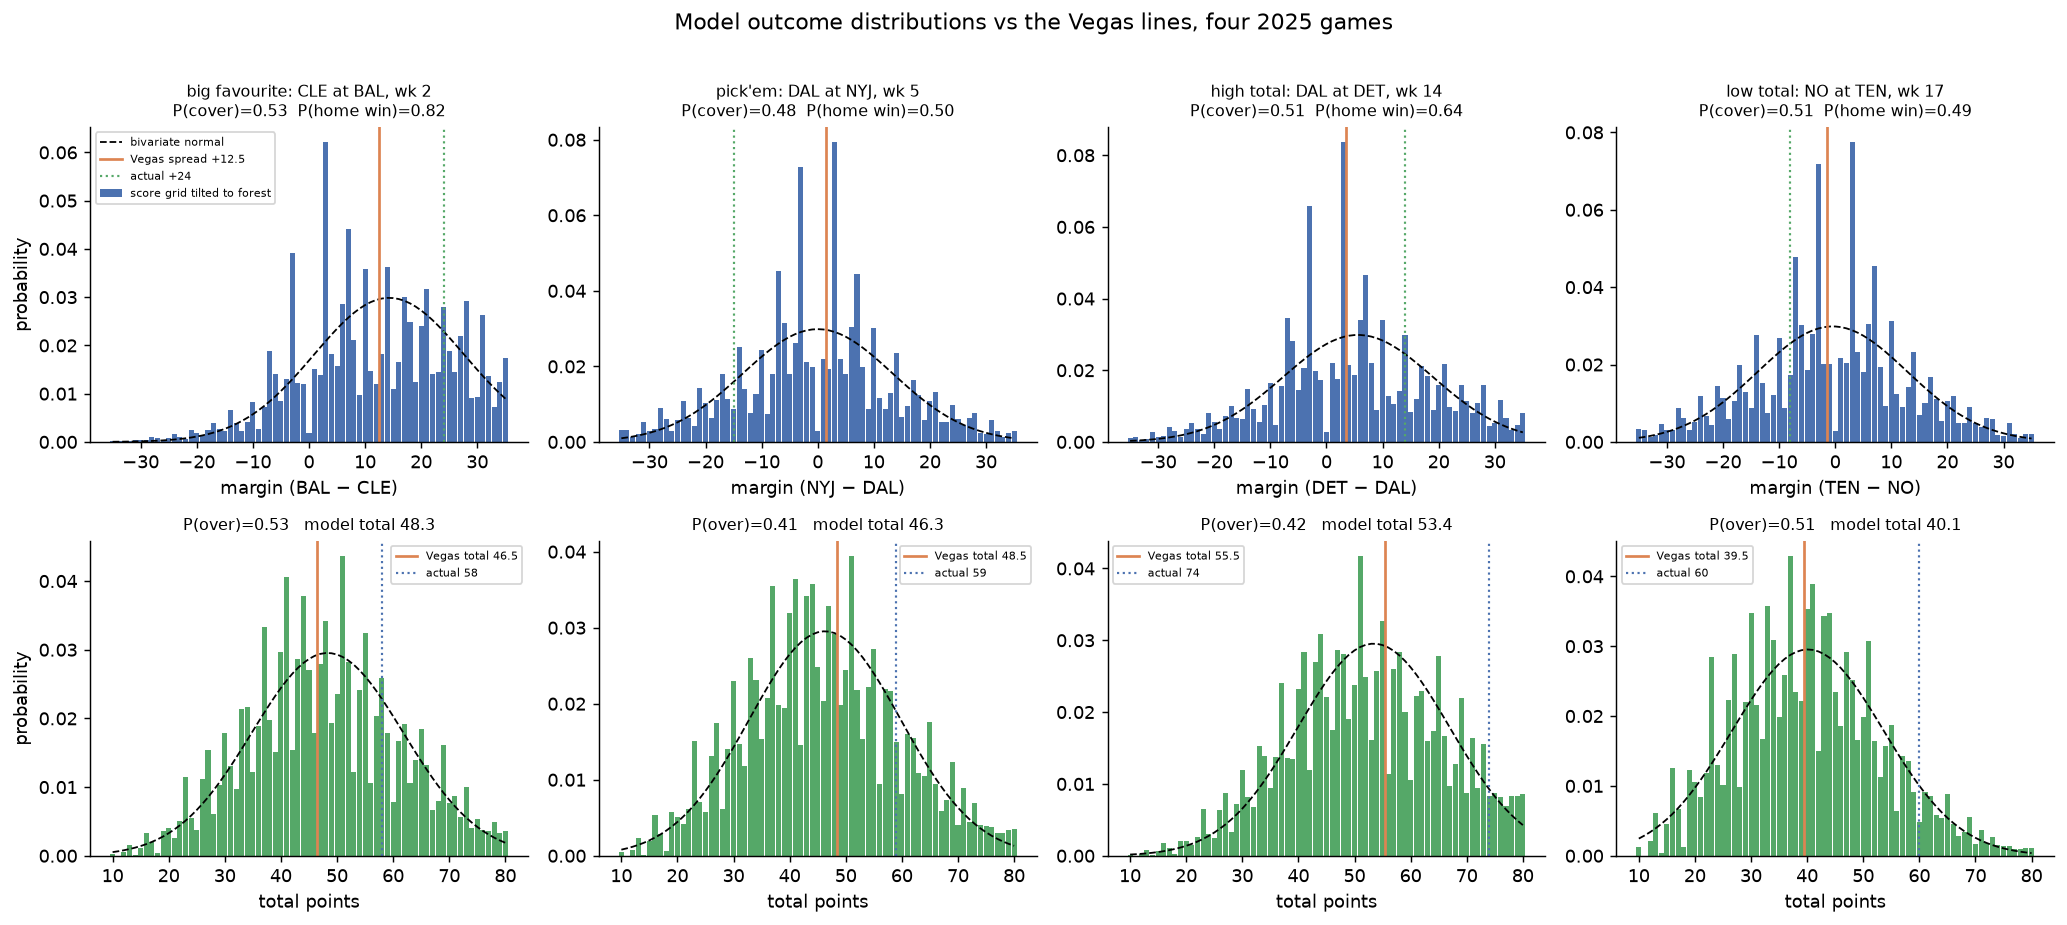
\includegraphics[width=\textwidth]{game_distributions.png}
\caption{Four 2025 games. Top: margin distribution from the tilted score grid (bars) and the bivariate normal (dashed), with the Vegas spread (orange) and the actual margin (dotted). Bottom: the same for the total.}
\label{fig:gamedist}
\end{figure}

\paragraph{How the calibration is measured.} For every game of 2016--2025 the empirical grid, with its prior built from the seasons before the test season, is tilted so that its mean margin and total equal the forest's two predictions; the model's probability of an event is the mass of that grid on the event's region. Games are then grouped by predicted probability in bins of width 0.1, and the observed frequency of the event in each bin is plotted against the mean prediction (Figures~\ref{fig:coverover} and~\ref{fig:fixedcal}). A forecast is calibrated if the points lie on the diagonal; it is informative if the predictions spread out along it. The Brier score summarises both, and we compare it with the climatological forecast that assigns every game the base rate.

\paragraph{Thresholds set by the market.} Across all 2,758 games the model's $P(\text{cover})$ averages 0.50 with a standard deviation of 0.09 and $P(\text{over})$ averages 0.49 with a standard deviation of 0.08; only a quarter of games get a cover probability outside 0.40--0.60. The calibration of these probabilities against outcomes is flat (Figure~\ref{fig:coverover}): when the model says 65\% to cover, teams cover about 52\%, and the regression slope of outcome on prediction is 0.06 for cover and 0.11 for over. Brier scores of 0.257 for cover and 0.255 for over are slightly worse than the 0.250 of the base rate. So, relative to the threshold the market has chosen, the model's probabilities carry no information. This is not a failure of calibration in the usual sense; it is what an efficient line implies. The closing spread is the market's median for the margin, set with everything the market knows, so conditioning on it removes exactly the part of the model's information that the market already has, and what remains is noise.

{\color{red}\textbf{Amine comment:} Please clarify how calibration is done. When the model predicts a 65\% chance of covering, the observed rate is about 52\%. Please also test fixed thresholds chosen in advance, separately from thresholds set by the market.}

{\color{blue}\textbf{Sai comment:} Fixed. The paragraph ``How the calibration is measured'' above states the procedure. The paragraph ``Thresholds fixed in advance'' below, with Table~\ref{tab:fixedcal} and Figure~\ref{fig:fixedcal}, tests seven pre-chosen events: the model has 8--11\% Brier skill on margin events and 3--4\% on totals with slopes 1.13--1.27, against slopes of 0.06--0.11 at the market's thresholds.}

\begin{figure}[H]
\centering
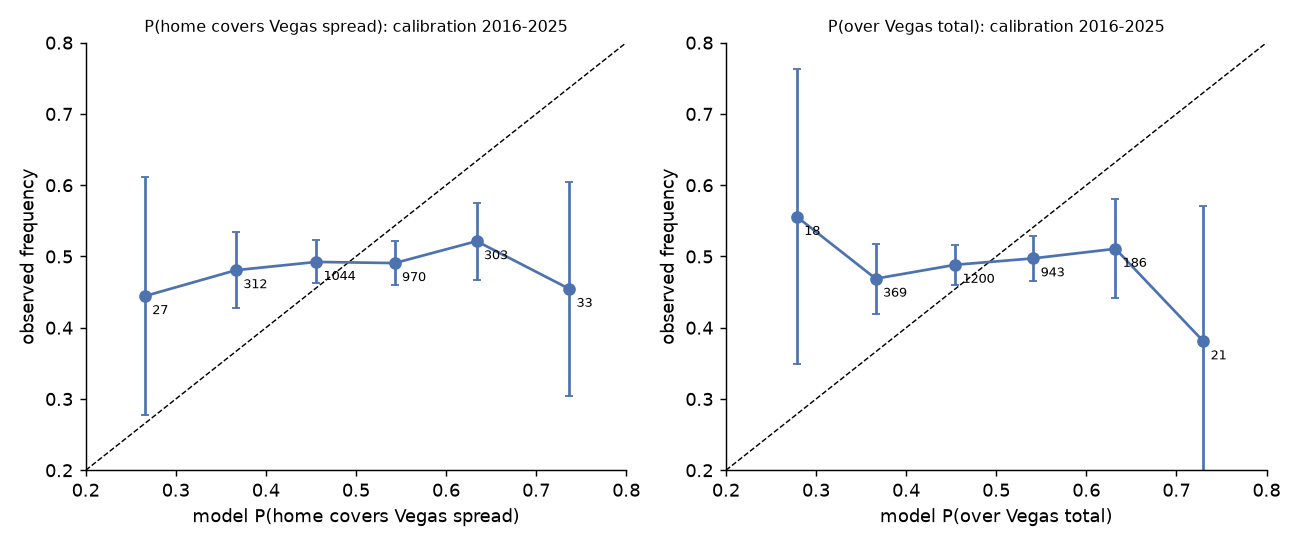
\includegraphics[width=0.95\textwidth]{cover_over_calibration.png}
\caption{Calibration of the model's cover and over probabilities against the closing line, 2016--2025; bin sizes shown.}
\label{fig:coverover}
\end{figure}

\paragraph{Thresholds fixed in advance.} The test Professor Amine asked for separates the two questions. We fixed seven thresholds before looking at the data, chosen to sit at round numbers and key numbers rather than at any game's line: the home team wins; wins by more than 3; by more than 7; the away team wins by more than 3; and the total exceeds 41, 45 and 48. For each the model probability is read from the same tilted grid, and the outcome is scored against the same 2,761 games (Table~\ref{tab:fixedcal}, Figure~\ref{fig:fixedcal}). At every fixed threshold the probabilities are informative: the Brier score beats the base rate by 8--11\% on the margin thresholds and 3--4\% on the totals, and the predictions spread across a range of 0.2 to 0.8. They are close to calibrated, with a regression slope of outcome on prediction between 1.13 and 1.27: the model is slightly under-confident, pushing its probabilities toward one half a little more than the outcomes warrant, which is the usual behaviour of a forest with large leaves. The totals carry less information than the margins (the predictions have a standard deviation of 0.08 against 0.13), consistent with the point-error table, where the model's total is further behind the line than its margin.

\begin{table}[H]
\centering
\small
\begin{tabular}{lcccccc}
\toprule
\textbf{Event} & \textbf{Base rate} & \textbf{SD of $p$} & \textbf{Brier} & \textbf{Brier, base rate} & \textbf{Skill} & \textbf{Slope} \\
\midrule
Home wins & 0.550 & 0.132 & 0.2212 & 0.2475 & 10.6\% & 1.25 \\
Home wins by $>3$ & 0.424 & 0.131 & 0.2182 & 0.2442 & 10.7\% & 1.27 \\
Home wins by $>7$ & 0.303 & 0.122 & 0.1915 & 0.2111 & 9.3\% & 1.18 \\
Away wins by $>3$ & 0.332 & 0.122 & 0.2032 & 0.2219 & 8.4\% & 1.13 \\
Total $>41$ & 0.595 & 0.076 & 0.2330 & 0.2409 & 3.3\% & 1.20 \\
Total $>45$ & 0.481 & 0.079 & 0.2406 & 0.2497 & 3.6\% & 1.24 \\
Total $>48$ & 0.396 & 0.077 & 0.2312 & 0.2391 & 3.3\% & 1.16 \\
\midrule
Home covers the closing spread & 0.493 & 0.088 & 0.2568 & 0.2499 & $-2.8\%$ & 0.06 \\
Over the closing total & 0.490 & 0.080 & 0.2550 & 0.2499 & $-2.0\%$ & 0.11 \\
\bottomrule
\end{tabular}
\caption{Model probabilities from the tilted grid scored against outcomes, 2016--2025 (2,761 games; ties excluded where they occur). Skill is one minus the ratio of the Brier score to that of the base-rate forecast; slope is the least-squares slope of the outcome on the prediction, 1 for a calibrated forecast.}
\label{tab:fixedcal}
\end{table}

\begin{figure}[H]
\centering
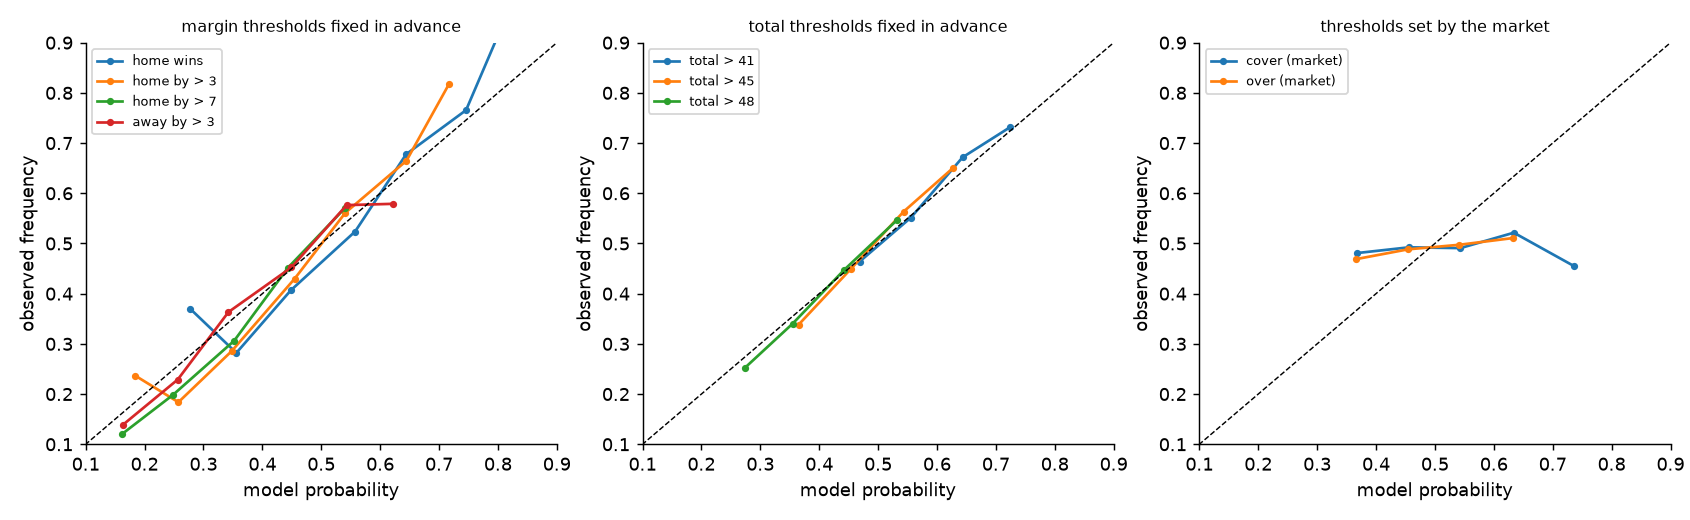
\includegraphics[width=\textwidth]{fixed_threshold_calibration.png}
\caption{Reliability of the model's probabilities at thresholds fixed in advance (left, centre) and at the thresholds set by the market (right), 2016--2025; bins with at least 30 games.}
\label{fig:fixedcal}
\end{figure}

The two tests together give the clean statement. The distributions are calibrated and informative for any event defined in advance, and carry nothing beyond what the closing line already contains for the event the line defines. The engine's value therefore lies in pricing the whole distribution consistently, not in picking sides against the market.

% ===== sections/conclusions.tex =====
\section{What we have learned, and next steps}

\subsection{What we have learned}
\begin{enumerate}[nosep]
\item For a binary contract, price, probability and the profit-and-loss distribution are the same thing; for a portfolio on one game, a joint distribution over the final score is the risk model. VaR and expected shortfall are then exact sums, with no covariance matrix or simulation.
\item The NFL score distribution is discrete in ways that matter for pricing: 3-point margins are 2.9 times as likely as a normal model says, and margin and total always share parity. An empirical score grid, repositioned by exponential tilting, prices a game's whole ladder of contracts to within a cent of the Kalshi order book once the dispersion is calibrated.
\item Point accuracy is capped near the Vegas closing line. Our two-output random forest, a linear model, Elo, a public Elo variant and every stack of them sit 0.1 to 0.4 points behind the line, as the literature has found since 1980. The forest and the linear model tie, so with 7,000 games the information is in the features, and the features are mostly ratings.
\item The forest's two score predictions are calibrated, and their residuals are uncorrelated with standard deviations near 9.5 points that rise with the level of scoring. Those are the parameters needed to turn two predicted scores into a probability for any outcome.
\item The resulting cover and over probabilities are calibrated for outcomes the market has not priced but carry no information about which side of the Vegas number will hit. The engine's value is in pricing the whole distribution consistently, not in picking sides against the market.
\item Leakage is the dominant risk in this kind of work and is easy to introduce from a well-maintained public dataset. A perturbation test and a sanity check against the literature's error levels are both needed.
\end{enumerate}

\subsection{Next steps}
\begin{enumerate}[nosep]
\item \textbf{Probabilistic head.} A model that predicts $(\mu_h,\mu_a,\sigma_h,\sigma_a,\rho)$ per game, trained on the bivariate negative log-likelihood, and used to position and scale the empirical grid. The toy example shows a dispersion parameter removes the remaining tail error.
\item \textbf{Remaining suggested methods} on the same feature table: LARS for a sparse linear model, gradient boosting, PCA and UMAP as exploration, and a cascade-correlation network as a final comparison.
\item \textbf{Offence and defence ratings} in the Glickman and Stern~\cite{glickmanstern1998} state-space form, so each predicted score has its own strength input rather than a single Elo; recency weighting for the scoring environment; a stadium lookup for travel distance.
\item \textbf{Risk layer.} Represent a book of Kalshi positions as a payoff vector on the score grid; compute ES, worst cell and probability of loss exactly; measure in-play jump risk from the trade tape, where hourly price changes are 17 cents against 1 cent pre-game; add the quoted-spread curve (which scales with $p(1-p)$, not with strike distance) as the liquidation cost.
\item \textbf{Live record.} Update weekly through the 2026 season: new games, new Kalshi prices, re-run the walk-forward, accumulate out-of-sample forecasts against the market.
\end{enumerate}



\bibliographystyle{plainnat}
\bibliography{riskpredictor}
\end{document}
